\stepcounter{section}
\section{Sudoku solver with simulated annealing}
\subsection{}
Appendix \ref{app: E 10} shows the code that solves a sudoku with simulated annealing.
\subsection{}
The main parameters that we can very is the starting $\beta: \beta_0$, the final beta $\beta_f$and the rate of change for $\beta: \delta \beta$. Every update step we update the temprature:
\begin{equation*}
    \centering
    \beta_{n +1} = \beta_n * \delta \beta
\end{equation*}

We choose our $\delta \beta$ such the in our $M_{steps}$we reach our $\beta_f$:
\begin{align*}
    \delta \beta = \left ( \frac{\beta_f}{\beta_0} \right )^{M_{check}/M_{steps}}.
\end{align*}
We update the $\beta$ every $M_{check}$ steps.\\
If we start of with a lower $\beta_0$ the simulation takes longer to converge but has a higer change of finding the right solution.
we choose $\beta_0$ such that we start of with an acceptence rate of about 0.5 meaning that half of the trail moves are accepted and we dont waste to much time at the start but have a high change of finding the right solution.
Four our sudoku's this comes down to a $\beta_0$ of 0.4 -1.0 depending on the sudoku puzzle.
We want to choose our $\delta \beta$ such that we slowly reach freezing at the and of the simulation. 
We choose a final $\beta_f$ of 20 so we get a rate of change of aboutn 1.015 so about $1.5 \% $.

We have tested it out for the easy and hard daily sudoku of the new york times. We see that the hard ones takes about twice as many steps.
But becuase of the random nature of our algoritme this may vary.
\subsection{}

\begin{figure}[H]
    \centering
    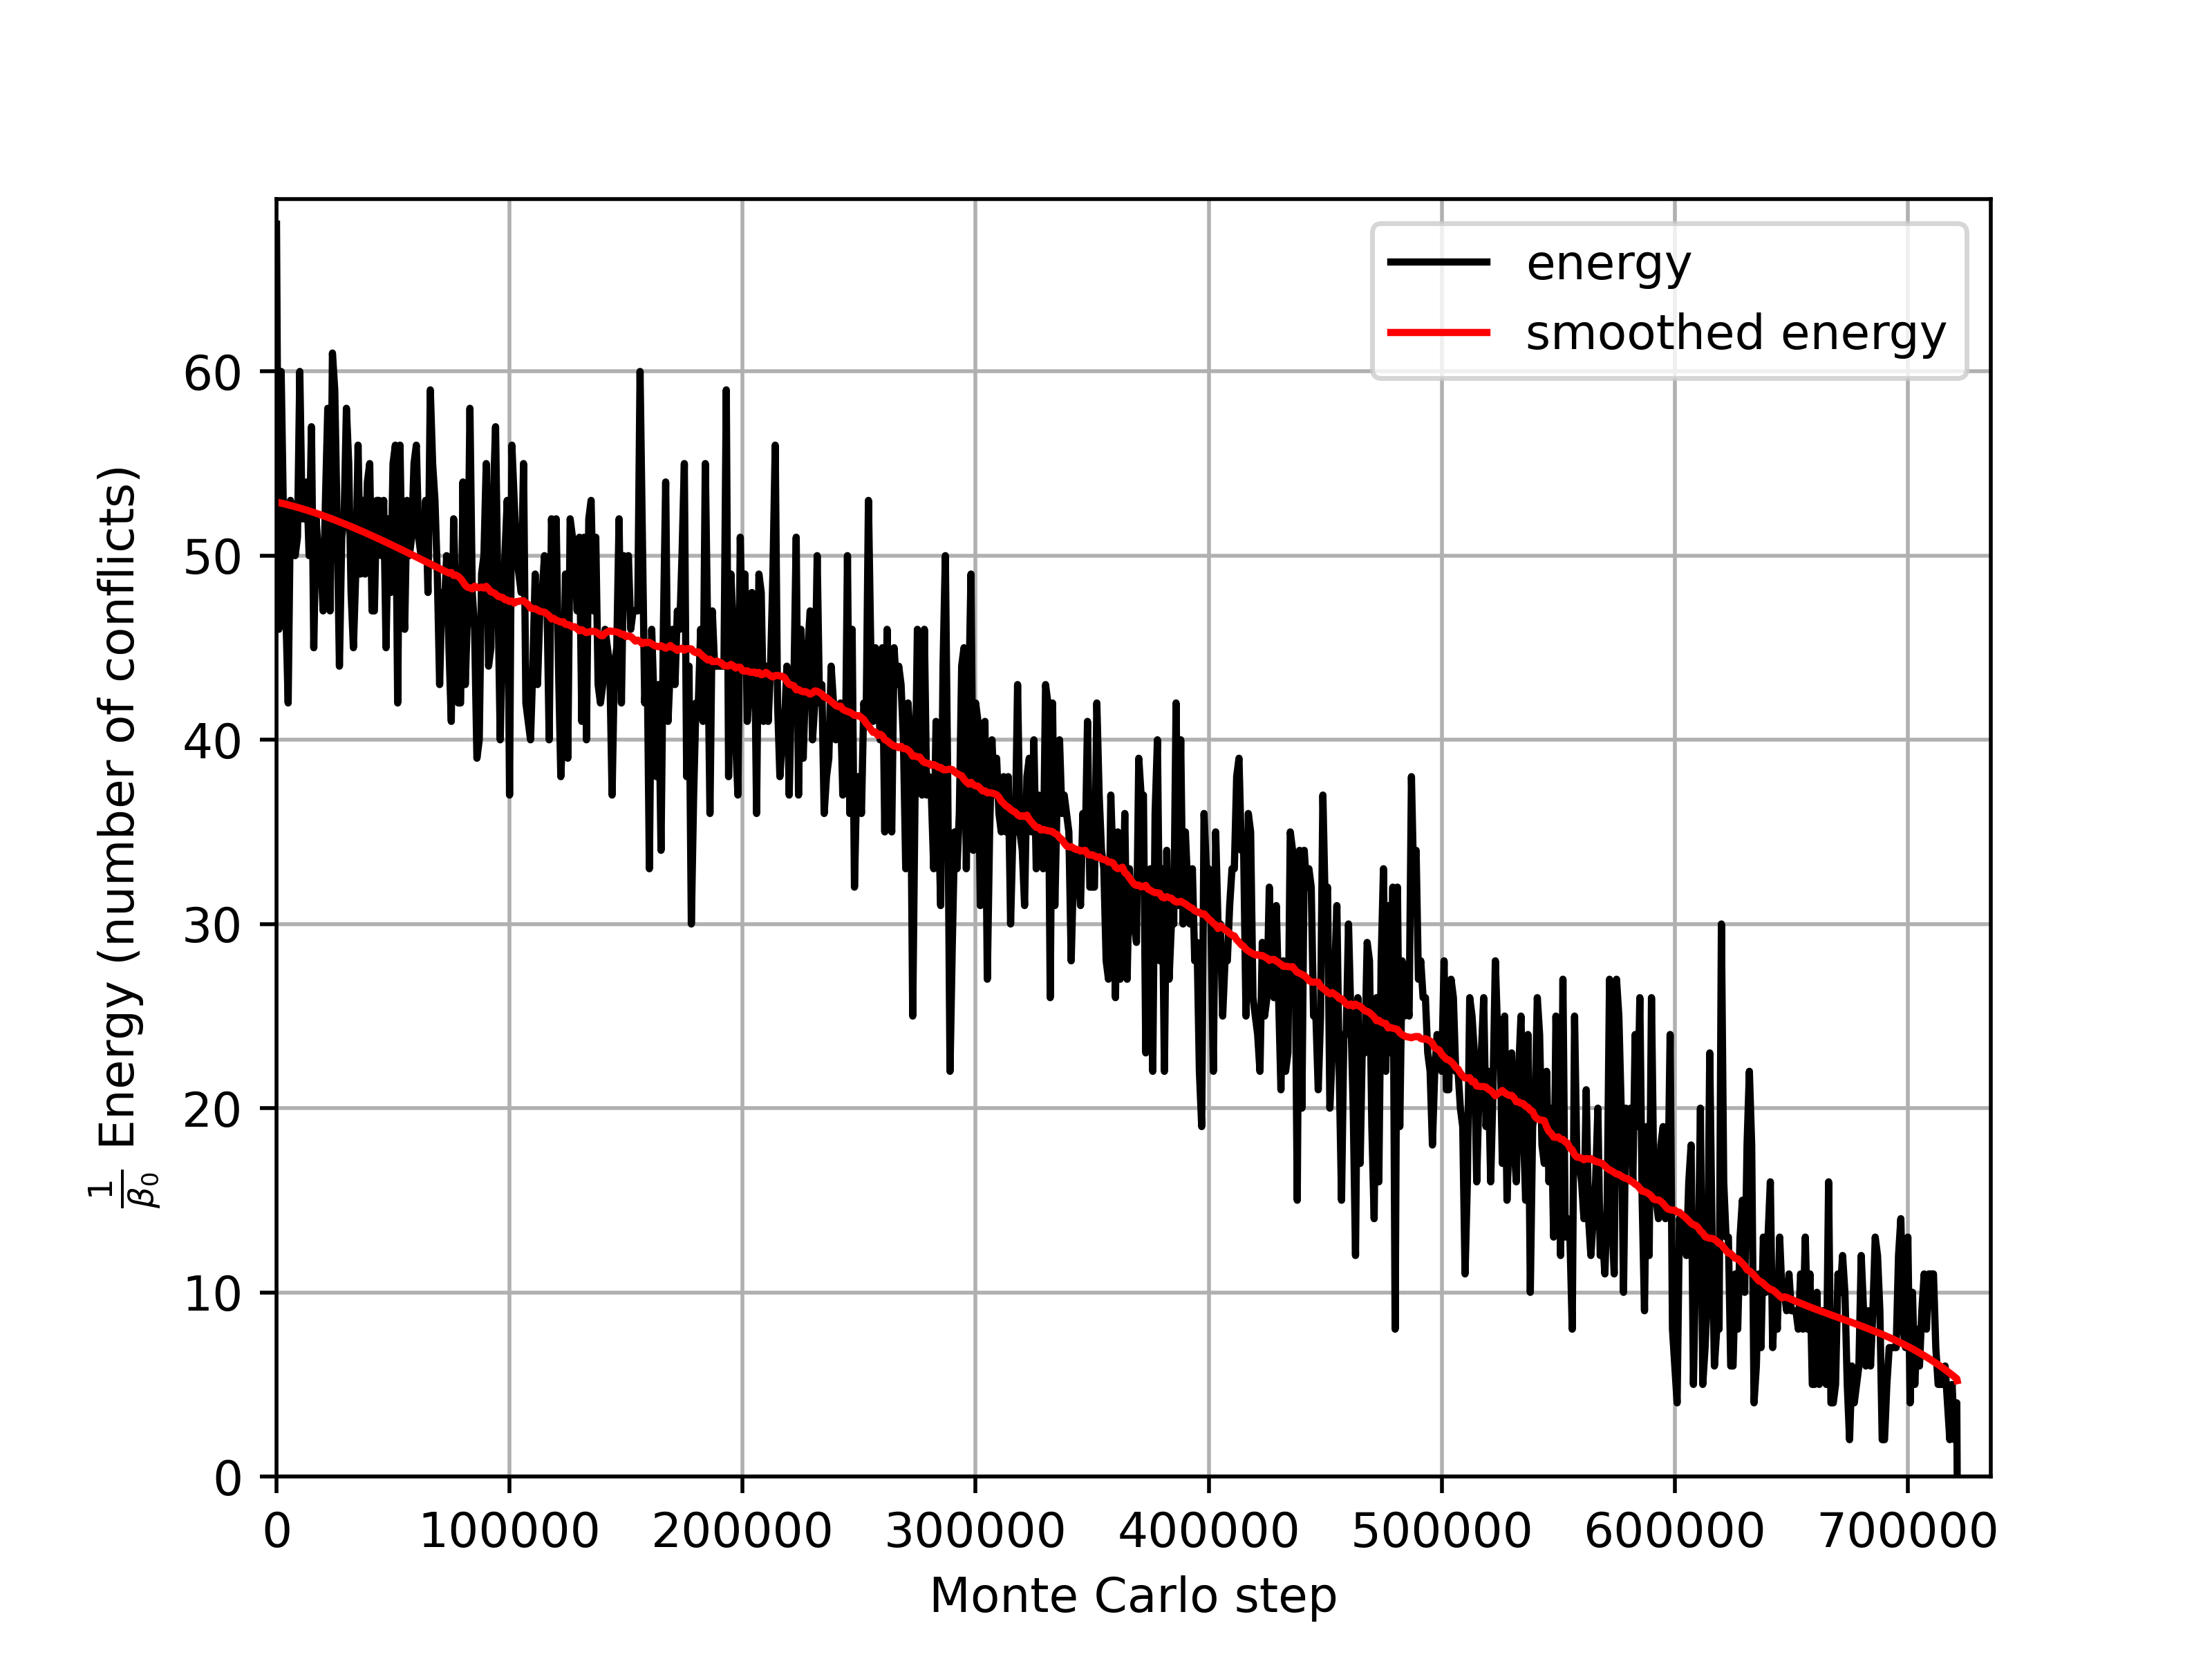
\includegraphics[width=1\linewidth]{graphs/E10/sudoku.png}
    \caption{ The energy (amount of conflicts) against the steps.}
    \label{fig: sudoku}
\end{figure}

\begin{figure}[H]
    \centering
    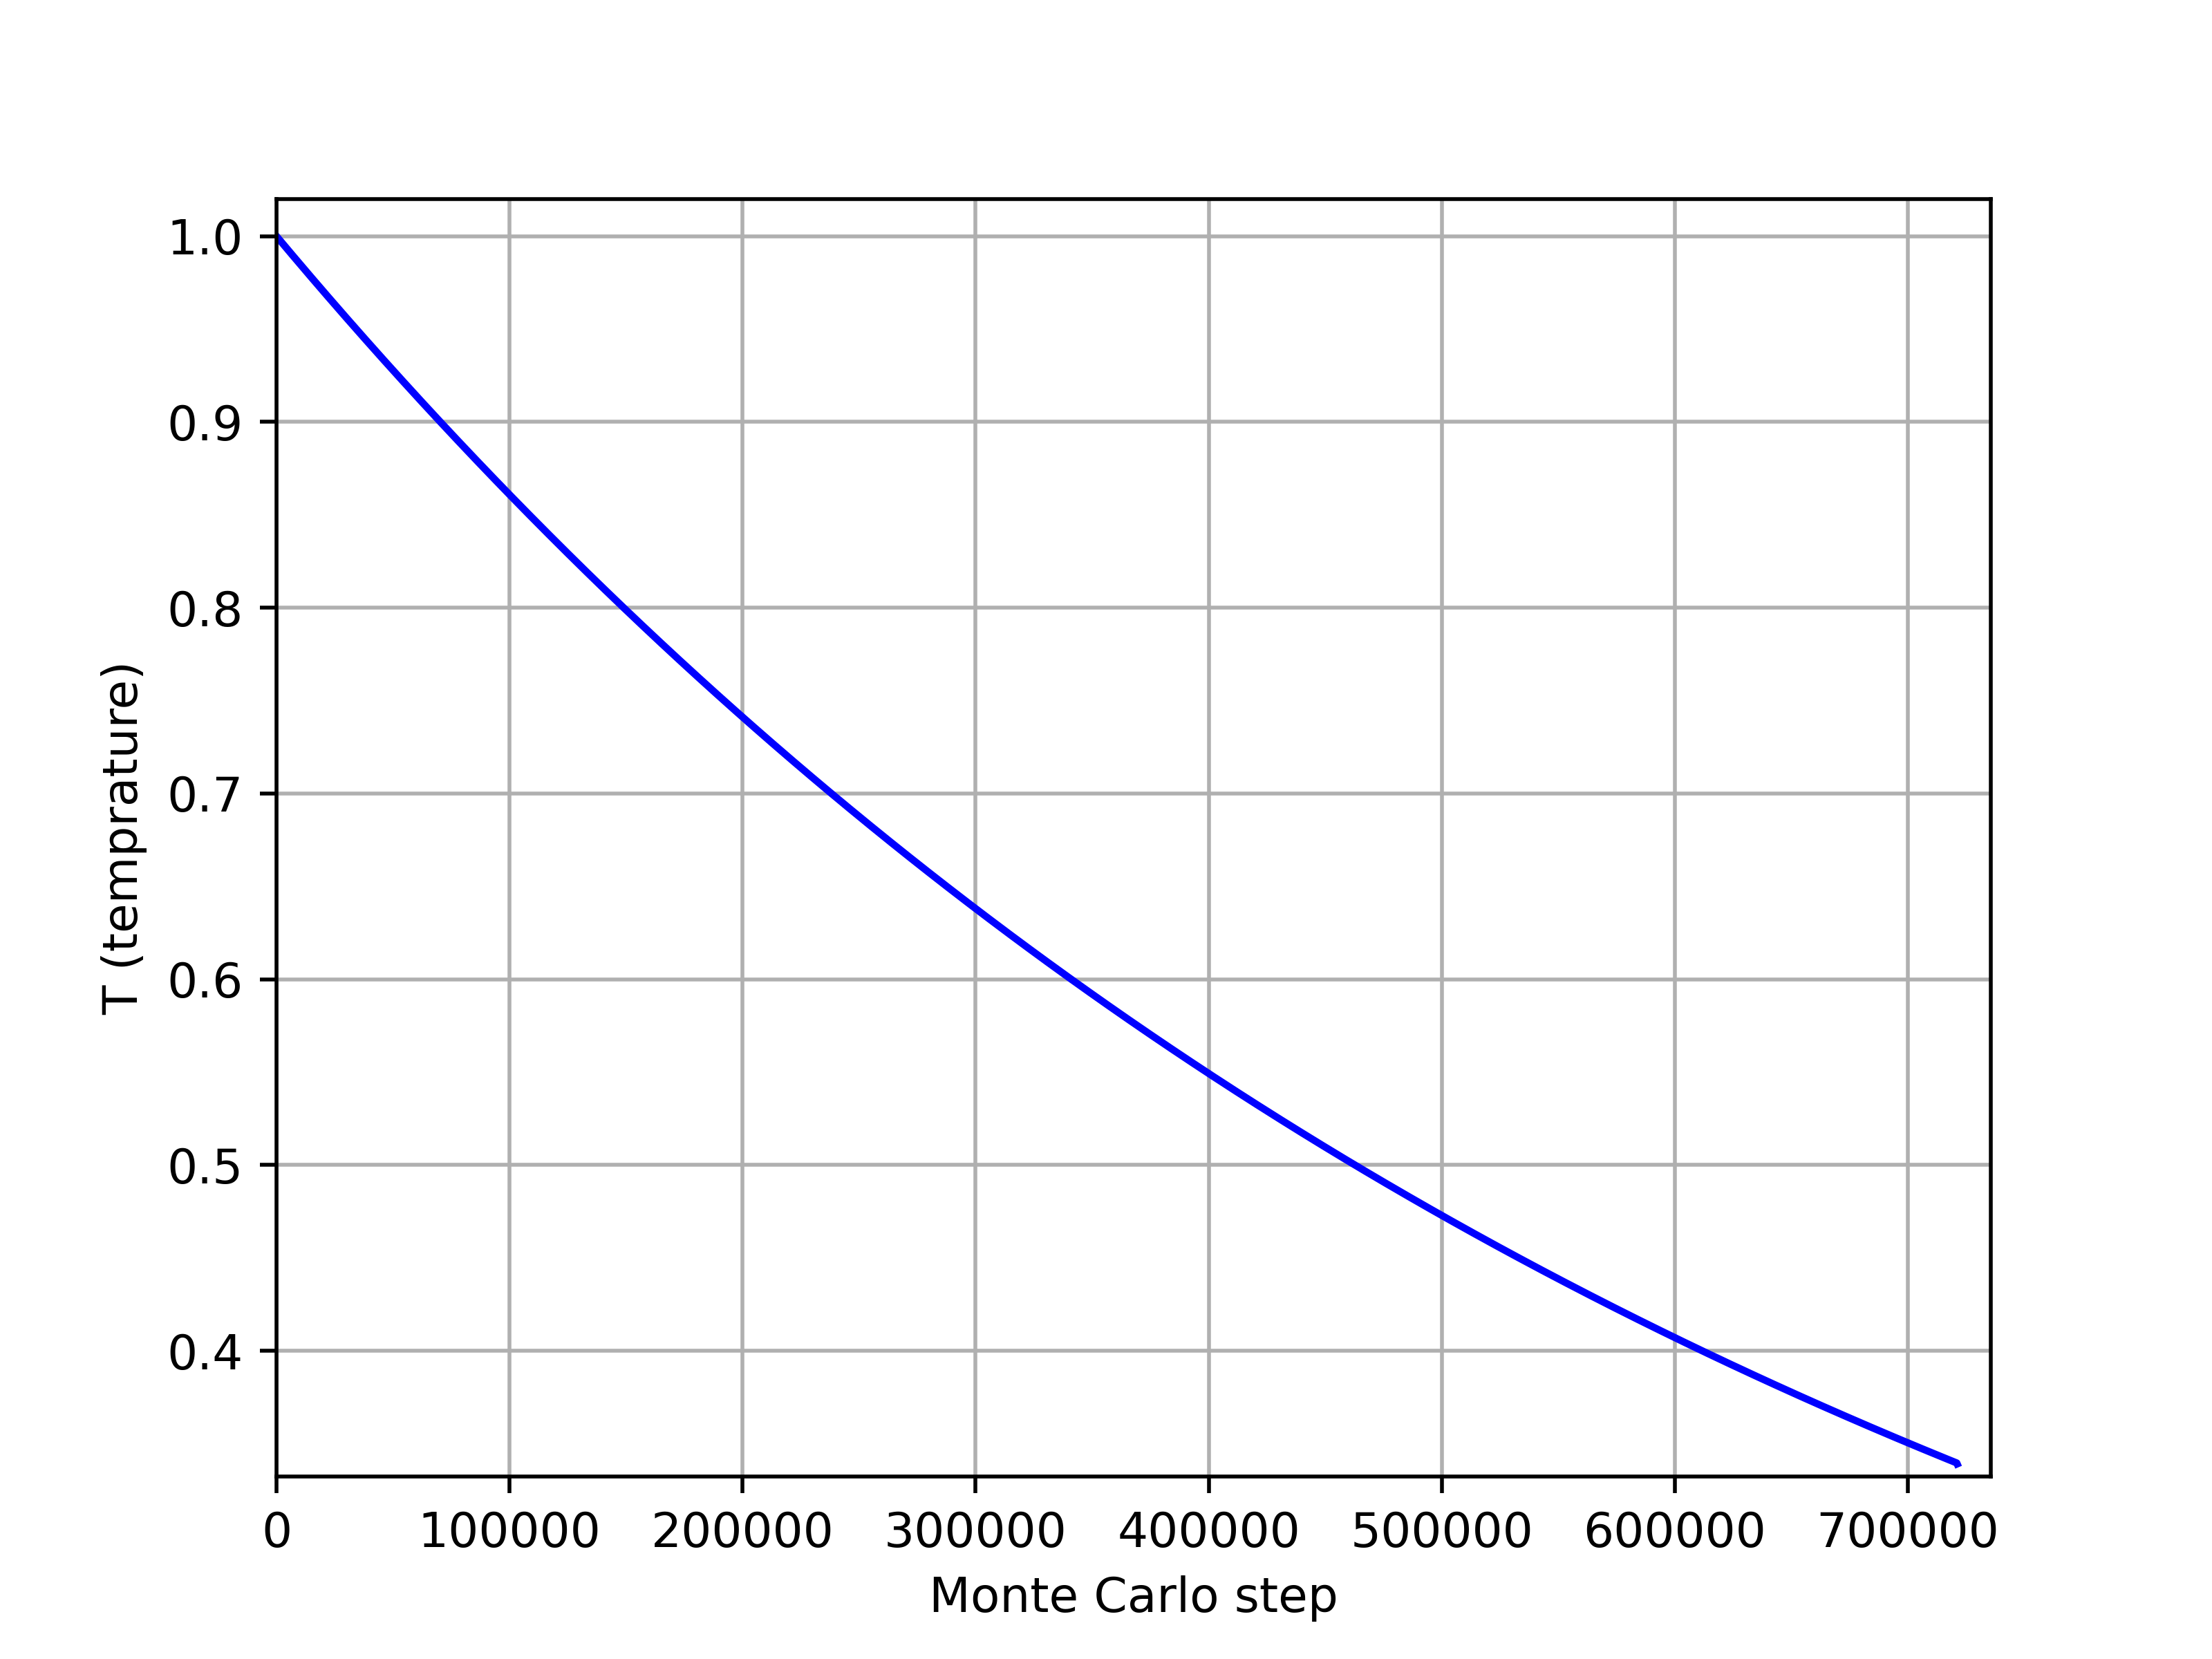
\includegraphics[width=1\linewidth]{graphs/E10/sudoku_temp.png}
    \caption{ The temprature against the steps.}
    \label{fig: sudoku_temp}
\end{figure}

In figure \ref{fig: sudoku} we see the energy in black has a generaldownward trend with noice making the graph jagged. 
We therfore used a salgov filter to smooth out the energy in red where we see the downward trend more clearly. 
In figure \ref{fig: sudoku_temp} we see that the temprature decreases exponential as expected from the formula we used for beta.

\subsection{}
There need to be 17 fixed squares to garanty a unique solution. This means that for our origional aproch there are:
$9^{64} \approx  10^{61}$ posible grids.

If we get an easier puzzle with more fixed squares the search space reduces.
This means that we are likely to find the solution sooner but becasue of our Monte Carlo simulation we are not garantueed to find a solution sooner.

The current aporoch of randomly filling the grid an changing a square to a random number is inefficient.
We can make use of the fact that we know that the grid contains every number 9 times and that every block contains every number. 
Instead of filling the grid completly random we can fill every block with all numbers from 1 to 9 after finding which numbers are missing in the puzzle. 
Instead of changing a random value we can then make random swaps within a block. this greatly reduces the searche space. 

For making swaps in a block with $k_b$ open squares there are $k_b !$ poabilites per block meaning there are a total of: $\prod_{b =1}^{9} k_b!$. 
If we assume there are 8 block with 7 open sqares and 1 with 8 there are $(7!)^8 8! \approx 10^{35}$ possible grids. 
This means we hve reduced our searche space by roughly a factor of $10^{27}$.

